\documentclass[11pt,a4paper,spanish]{book}
\usepackage{estilo_unir-1}
\hypersetup{
	colorlinks   = true,
	urlcolor     = blue,
	linkcolor    = black,
	citecolor    = red
}
\usepackage[nottoc]{tocbibind}
\usepackage{tikz}
\usetikzlibrary{arrows.meta, positioning, fit}
\usepackage{listings}
\usepackage{graphicx}
\lstset{
	basicstyle=\ttfamily\footnotesize,
	breaklines=true,
	frame=single,
	backgroundcolor=\color[gray]{0.95},
	numbers=left,
	numberstyle=\tiny\color[gray]{0.5},
	keywordstyle=\color{blue},
	commentstyle=\color[gray]{0.5},
	tabsize=2
}

%---------------------------
% Datos del trabajo
%---------------------------
\subject{Pr\'{a}cticas Acad\'{e}micas Externas}
\title{Sistema de medici\'{o}n de impedancia (EIS) para cuantificaci\'{o}n de Candida albicans --- Fase 4}
\author{Andr\'{e}s Alexandro Tapia Flores}
\profesor{Universidad Internacional de la Rioja (UNIR)}
\date{Abril 2026}

\begin{document}
\renewcommand{\listfigurename}{\'{I}ndice de figuras}
\renewcommand{\contentsname}{\'{I}ndice de contenidos}
\renewcommand{\figurename}{Figura}
\renewcommand{\tablename}{Tabla}
\setlength{\headheight}{26pt}

\maketitle
\frontmatter
\tableofcontents

\chapter{Resumen}
La Fase~4 se centra en el registro persistente de datos de adquisici\'{o}n, el almacenamiento de metadatos por sesi\'{o}n, la exportaci\'{o}n estructurada de resultados y la trazabilidad de clasificaci\'{o}n cu\'{a}ntica/cl\'{a}sica para comparaci\'{o}n en interfaz.

Se implementa un modelo de sesi\'{o}n en backend que encapsula configuraci\'{o}n, calibraci\'{o}n, temperatura, datos punto a punto, eventos de protocolo y salida de clasificadores. Cada barrido finalizado genera artefactos exportables en formatos complementarios (CSV, JSON y resumen textual), permitiendo auditor\'{i}a t\'{e}cnica y uso posterior en pipelines de aprendizaje.

\vspace{0.5cm}
{\bf Palabras clave:} registro de datos, metadatos, exportaci\'{o}n, trazabilidad, clasificaci\'{o}n cu\'{a}ntica

\mainmatter

\chapter{Introducci\'{o}n}

Una etapa cr\'{i}tica del sistema EIS no es solo adquirir y visualizar, sino conservar cada sesi\'{o}n con contexto suficiente para su reproducci\'{o}n anal\'{i}tica. En aplicaciones bioelectroqu\'{i}micas, la interpretaci\'{o}n posterior requiere conocer condiciones de barrido, estado de calibraci\'{o}n, temperatura, etiqueta objetivo y comportamiento del clasificador.

En esta fase se implementa una capa de persistencia orientada a sesiones, de forma que cada barrido se convierte en una unidad trazable y exportable. Este enfoque permite:
\begin{itemize}
	\item Integraci\'{o}n con entrenamiento de modelos (cu\'{a}nticos y cl\'{a}sicos).
	\item Auditor\'{i}a de calidad de adquisici\'{o}n.
	\item Comparaci\'{o}n temporal entre ejecuciones.
	\item Reproducibilidad de experimentos.
\end{itemize}


\chapter{Objetivos}

\section{Objetivo general}
Dise\~{n}ar e implementar el subsistema de registro, metadatos y exportaci\'{o}n para sesiones de adquisici\'{o}n EIS, incorporando resultado de clasificaci\'{o}n cu\'{a}ntica y comparaci\'{o}n con clasificador cl\'{a}sico.

\section{Objetivos espec\'{i}ficos}
\begin{itemize}
	\item Definir un modelo de sesi\'{o}n persistente para cada barrido.
	\item Almacenar datos crudos y eventos de protocolo con marcas temporales UTC.
	\item Asociar metadatos de configuraci\'{o}n, calibraci\'{o}n y temperatura.
	\item Exportar datos en m\'{u}ltiples formatos para consumo anal\'{i}tico.
	\item Exponer en UI la ruta de exportaci\'{o}n y el historial de sesiones.
	\item Verificar consistencia entre etiqueta esperada y etiqueta predicha por modelos cu\'{a}ntico y cl\'{a}sico.
\end{itemize}


\chapter{Dise\~{n}o del registro y metadatos}

\section{Entidad de sesi\'{o}n}

Cada barrido se modela como una sesi\'{o}n con identificador \texttt{session\_<timestamp>}. Incluye:
\begin{itemize}
	\item Identidad temporal: inicio, fin y motivo de cierre.
	\item Contexto instrumental: configuraci\'{o}n de barrido, calibraci\'{o}n y temperatura.
	\item Datos: secuencia de puntos EIS con timestamp individual.
	\item Eventos: \texttt{sweep\_start}, \texttt{sweep\_done}, errores y se\~{n}ales de control.
	\item Resultado anal\'{i}tico: probabilidad/etiqueta cu\'{a}ntica, probabilidad/etiqueta cl\'{a}sica y campos de coincidencia.
\end{itemize}

\section{Flujo de persistencia}

El flujo implementado se resume en la Figura~\ref{fig:persistencia-fase4}.

\begin{figure}[ht]
	\centering
	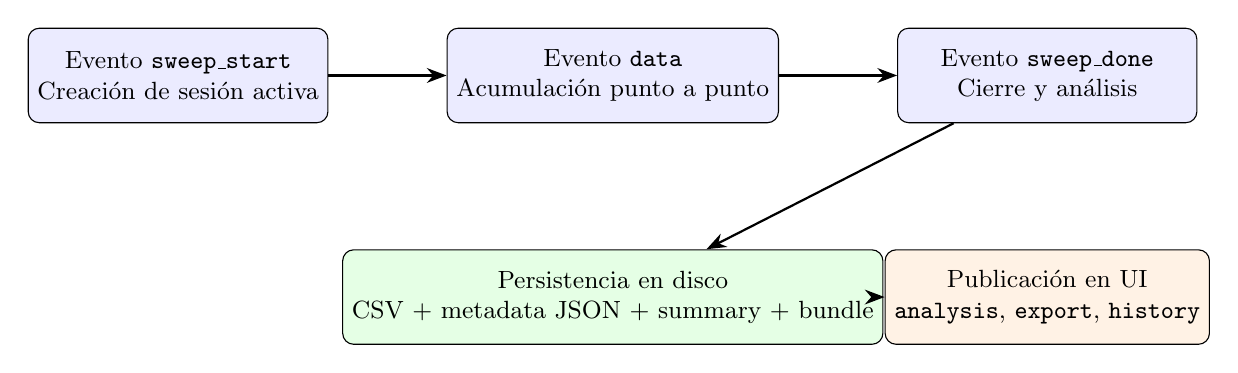
\begin{tikzpicture}[
		node distance=1.6cm and 1.5cm,
		block/.style={rectangle, draw, rounded corners, fill=blue!8, minimum width=3.8cm, minimum height=1.2cm, align=center, font=\small},
		arrow/.style={-{Stealth[length=2.5mm]}, thick}
		]
		\node[block] (start) {Evento \texttt{sweep\_start}\\Creaci\'{o}n de sesi\'{o}n activa};
		\node[block, right=of start] (data) {Evento \texttt{data}\\Acumulaci\'{o}n punto a punto};
		\node[block, right=of data] (close) {Evento \texttt{sweep\_done}\\Cierre y an\'{a}lisis};
		\node[block, below=of data, fill=green!10] (files) {Persistencia en disco\\CSV + metadata JSON + summary + bundle};
		\node[block, below=of close, fill=orange!10] (ui) {Publicaci\'{o}n en UI\\\texttt{analysis}, \texttt{export}, \texttt{history}};

		\draw[arrow] (start) -- (data);
		\draw[arrow] (data) -- (close);
		\draw[arrow] (close) -- (files);
		\draw[arrow] (files) -- (ui);
	\end{tikzpicture}
	\caption[Flujo de persistencia por sesi\'{o}n]{Flujo de registro en backend para cierre de sesi\'{o}n y exportaci\'{o}n. Fuente: elaboraci\'{o}n propia.}
	\label{fig:persistencia-fase4}
\end{figure}

\section{Estructura de salida}

Por cada sesi\'{o}n se crea un directorio en \texttt{data/acquisitions/<session\_id>/} con los siguientes archivos:

\begin{table}[ht]
	\centering
	\begin{tabular}{l p{8.8cm}}
		\hline\hline
		Archivo                      & Contenido                                                                 \\ [0.5ex]
		\hline
		\texttt{<id>\_data.csv}      & Puntos EIS crudos con columnas \texttt{i,f,Z,phase,reZ,imZ,ts}.           \\
		\texttt{<id>\_metadata.json} & Metadatos de sesi\'{o}n, eventos y resultado de clasificaci\'{o}n.        \\
		\texttt{<id>\_summary.txt}   & Resumen textual compacto para inspecci\'{o}n r\'{a}pida en consola.       \\
		\texttt{<id>\_bundle.json}   & Paquete integral (metadatos + puntos + eventos) para intercambio directo. \\
		\hline
	\end{tabular}
	\caption[Artefactos de exportaci\'{o}n]{Artefactos generados por sesi\'{o}n al finalizar un barrido. Fuente: elaboraci\'{o}n propia.}
	\label{tab:artefactos-fase4}
\end{table}


\chapter{Algoritmo clasificador cu\'{a}ntico y verificaci\'{o}n en UI}

\section{Implementaci\'{o}n del clasificador cu\'{a}ntico}

El clasificador cu\'{a}ntico se implementa en \texttt{src/classifier.py} como un simulador vectorial de estado para 4 qubits, con las siguientes etapas:

\begin{enumerate}
	\item \textbf{Extracci\'{o}n de caracter\'{i}sticas}: media de magnitud, pendiente logar\'{i}tmica, energ\'{i}a imaginaria, rango de fase, desviaci\'{o}n de fase y raz\'{o}n baja/alta frecuencia.
	\item \textbf{Normalizaci\'{o}n}: mapeo de cada descriptor a $[-1,1]$ por funci\'{o}n \texttt{tanh} calibrada.
	\item \textbf{Codificaci\'{o}n angular}: transformaci\'{o}n de descriptores en \textit{angles} para rotaciones $R_Y$.
	\item \textbf{Ansatz variacional}: capas $R_Y$, $R_Z$ y compuertas CNOT en topolog\'{i}a anillo/parcial.
	\item \textbf{Medici\'{o}n}: c\'{a}lculo de valores esperados en qubits 0 y 2, combinados con un t\'{e}rmino de \textit{feature drive} para obtener score final.
\end{enumerate}

\subsection{Normalizaci\'{o}n de caracter\'{i}sticas}

Cada descriptor se normaliza al rango $[-1, 1]$ mediante $\tanh(\cdot)$ centrado en la frontera emp\'{i}rica entre clases y con una escala proporcional a la separaci\'{o}n t\'{i}pica entre Control y Candida. Los centros y escalas se derivan de un circuito de Randles simulado ($R_s$ + $R_{ct} \parallel C_{dl}$ + Warburg) con par\'{a}metros distintos para cada clase; la Tabla~\ref{tab:randles-params} resume los valores empleados durante la simulaci\'{o}n.

\begin{table}[ht]
	\centering
	\begin{tabular}{l r r}
		\hline\hline
		Par\'{a}metro     & Control (label 0) & Candida (label 1) \\ [0.5ex]
		\hline
		$R_s$ ($\Omega$)  & 310               & 220               \\
		$R_{ct}$ ($\Omega$) & 11500           & 7200              \\
		$C_{dl}$ (F)      & $1.9\times 10^{-6}$ & $3.2\times 10^{-6}$ \\
		$\sigma$ Warburg  & 250               & 420               \\
		\hline
	\end{tabular}
	\caption[Par\'{a}metros de Randles por clase]{Par\'{a}metros del circuito equivalente de Randles utilizados por la simulaci\'{o}n para generar las clases de referencia. Fuente: elaboraci\'{o}n propia.}
	\label{tab:randles-params}
\end{table}

Los centros y escalas que aplica \texttt{tanh} a cada feature se eligen como punto medio entre los valores t\'{i}picos de cada clase (centro) y aproximadamente la mitad de la separaci\'{o}n (escala), tal como se detalla en la Tabla~\ref{tab:features-norm}.

\begin{table}[ht]
	\centering
	\scriptsize
	\begin{tabular}{l c c c c}
		\hline\hline
		Feature                 & Valor t\'{i}pico Control & Valor t\'{i}pico Candida & Centro & Escala \\ [0.5ex]
		\hline
		\texttt{mag\_mean}      & 330 $\Omega$           & 230 $\Omega$             & 270    & 85     \\
		\texttt{mag\_slope}     & $-4.1$                  & $-4.8$                   & $-4.4$ & 0.35   \\
		\texttt{im\_energy}     & 12 $\Omega$             & 22 $\Omega$              & 17     & 5      \\
		\texttt{phase\_span}    & $12^\circ$              & $17^\circ$               & 14.3   & 2.2    \\
		\texttt{phase\_std}     & $3.3^\circ$             & $4.6^\circ$              & 3.9    & 0.8    \\
		\texttt{low\_high\_ratio} & 1.018                 & 1.028                    & 1.022  & 0.01   \\
		\hline
	\end{tabular}
	\caption[Normalizaci\'{o}n de features]{Centros y escalas de normalizaci\'{o}n derivados del modelo de Randles simulado. Fuente: elaboraci\'{o}n propia.}
	\label{tab:features-norm}
\end{table}

\subsection{Codificaci\'{o}n angular y ansatz}

Las cuatro primeras features normalizadas (\texttt{mag\_mean\_norm}, \texttt{mag\_slope\_norm}, \texttt{im\_energy\_norm}, \texttt{phase\_span\_norm}) se convierten en \'{a}ngulos de rotaci\'{o}n mediante
\[
\theta_i = (f_i + 1)\,\frac{\pi}{2},
\]
que mapea $[-1, 1]$ a $[0, \pi]$ y se aplican como compuertas $R_Y(\theta_i)$ sobre los cuatro qubits, seguidas de CNOT en anillo ($0\!\rightarrow\!1\!\rightarrow\!2\!\rightarrow\!3\!\rightarrow\!0$). Posteriormente se ejecutan dos capas de rotaciones parametrizadas $R_Y$ + $R_Z$ con pesos preentrenados y CNOT adicionales.

\subsection{Medici\'{o}n y score}

Del estado cuantico final se miden los valores esperados $Z$ de los qubits 0 y 2 ($z_0$, $z_2$) y se combinan con un promedio ponderado de las seis features normalizadas:
\begin{align*}
\mathrm{feature\_drive} = &\ 0.35\,\mathrm{mag\_mean\_norm} + 0.25\,\mathrm{im\_energy\_norm} \\
&\ + 0.15\,\mathrm{phase\_span\_norm} + 0.10\,\mathrm{phase\_std\_norm} \\
&\ + 0.10\,\mathrm{mag\_slope\_norm} + 0.05\,\mathrm{low\_high\_ratio\_norm}, \\
\mathrm{score} = &\ \mathrm{clamp}(-0.35\,z_0 - 0.20\,z_2 + 0.45\,\mathrm{feature\_drive},\ -1,\ 1), \\
p_q = &\ (\mathrm{score} + 1)/2.
\end{align*}

La etiqueta cu\'{a}ntica es 1 (Candida) si $p_q \geq 0.5$, y 0 (Control) en caso contrario.

\section{Comparador cl\'{a}sico}

En paralelo se calcula una probabilidad cl\'{a}sica mediante regresi\'{o}n log\'{i}stica con pesos fijos sobre las seis features normalizadas:
\begin{align*}
\ell = &\ 1.60\,\mathrm{mag\_mean\_norm} + 0.70\,\mathrm{mag\_slope\_norm} \\
&\ + 1.20\,\mathrm{im\_energy\_norm} + 0.90\,\mathrm{phase\_span\_norm} \\
&\ + 0.80\,\mathrm{phase\_std\_norm} + 0.60\,\mathrm{low\_high\_ratio\_norm} + 0.05, \\
p_c = &\ \frac{1}{1 + e^{-\ell}}.
\end{align*}

La etiqueta cl\'{a}sica aplica el mismo umbral $0.5$. Este valor se usa como contraste operativo en la UI y como criterio de coherencia entre modelos.

\section{Verificaci\'{o}n de valor en interfaz}

La interfaz muestra por sesi\'{o}n:
\begin{itemize}
	\item Probabilidad cu\'{a}ntica y etiqueta cu\'{a}ntica.
	\item Probabilidad cl\'{a}sica y etiqueta cl\'{a}sica.
	\item Campo \texttt{expected\_label} y banderas \texttt{quantum\_match}/\texttt{classical\_match}.
	\item Estado de acuerdo/discrepancia entre modelos.
\end{itemize}

Esto satisface el requerimiento de comparaci\'{o}n expl\'{i}cita de valor clasificador en la UI. La Figura~\ref{fig:ui-analisis-fase4} muestra el panel de clasificaci\'{o}n al cierre de un barrido, incluyendo las seis features normalizadas y el campo de exportaci\'{o}n con las rutas de los artefactos generados autom\'{a}ticamente.

\begin{figure}[ht]
	\centering
	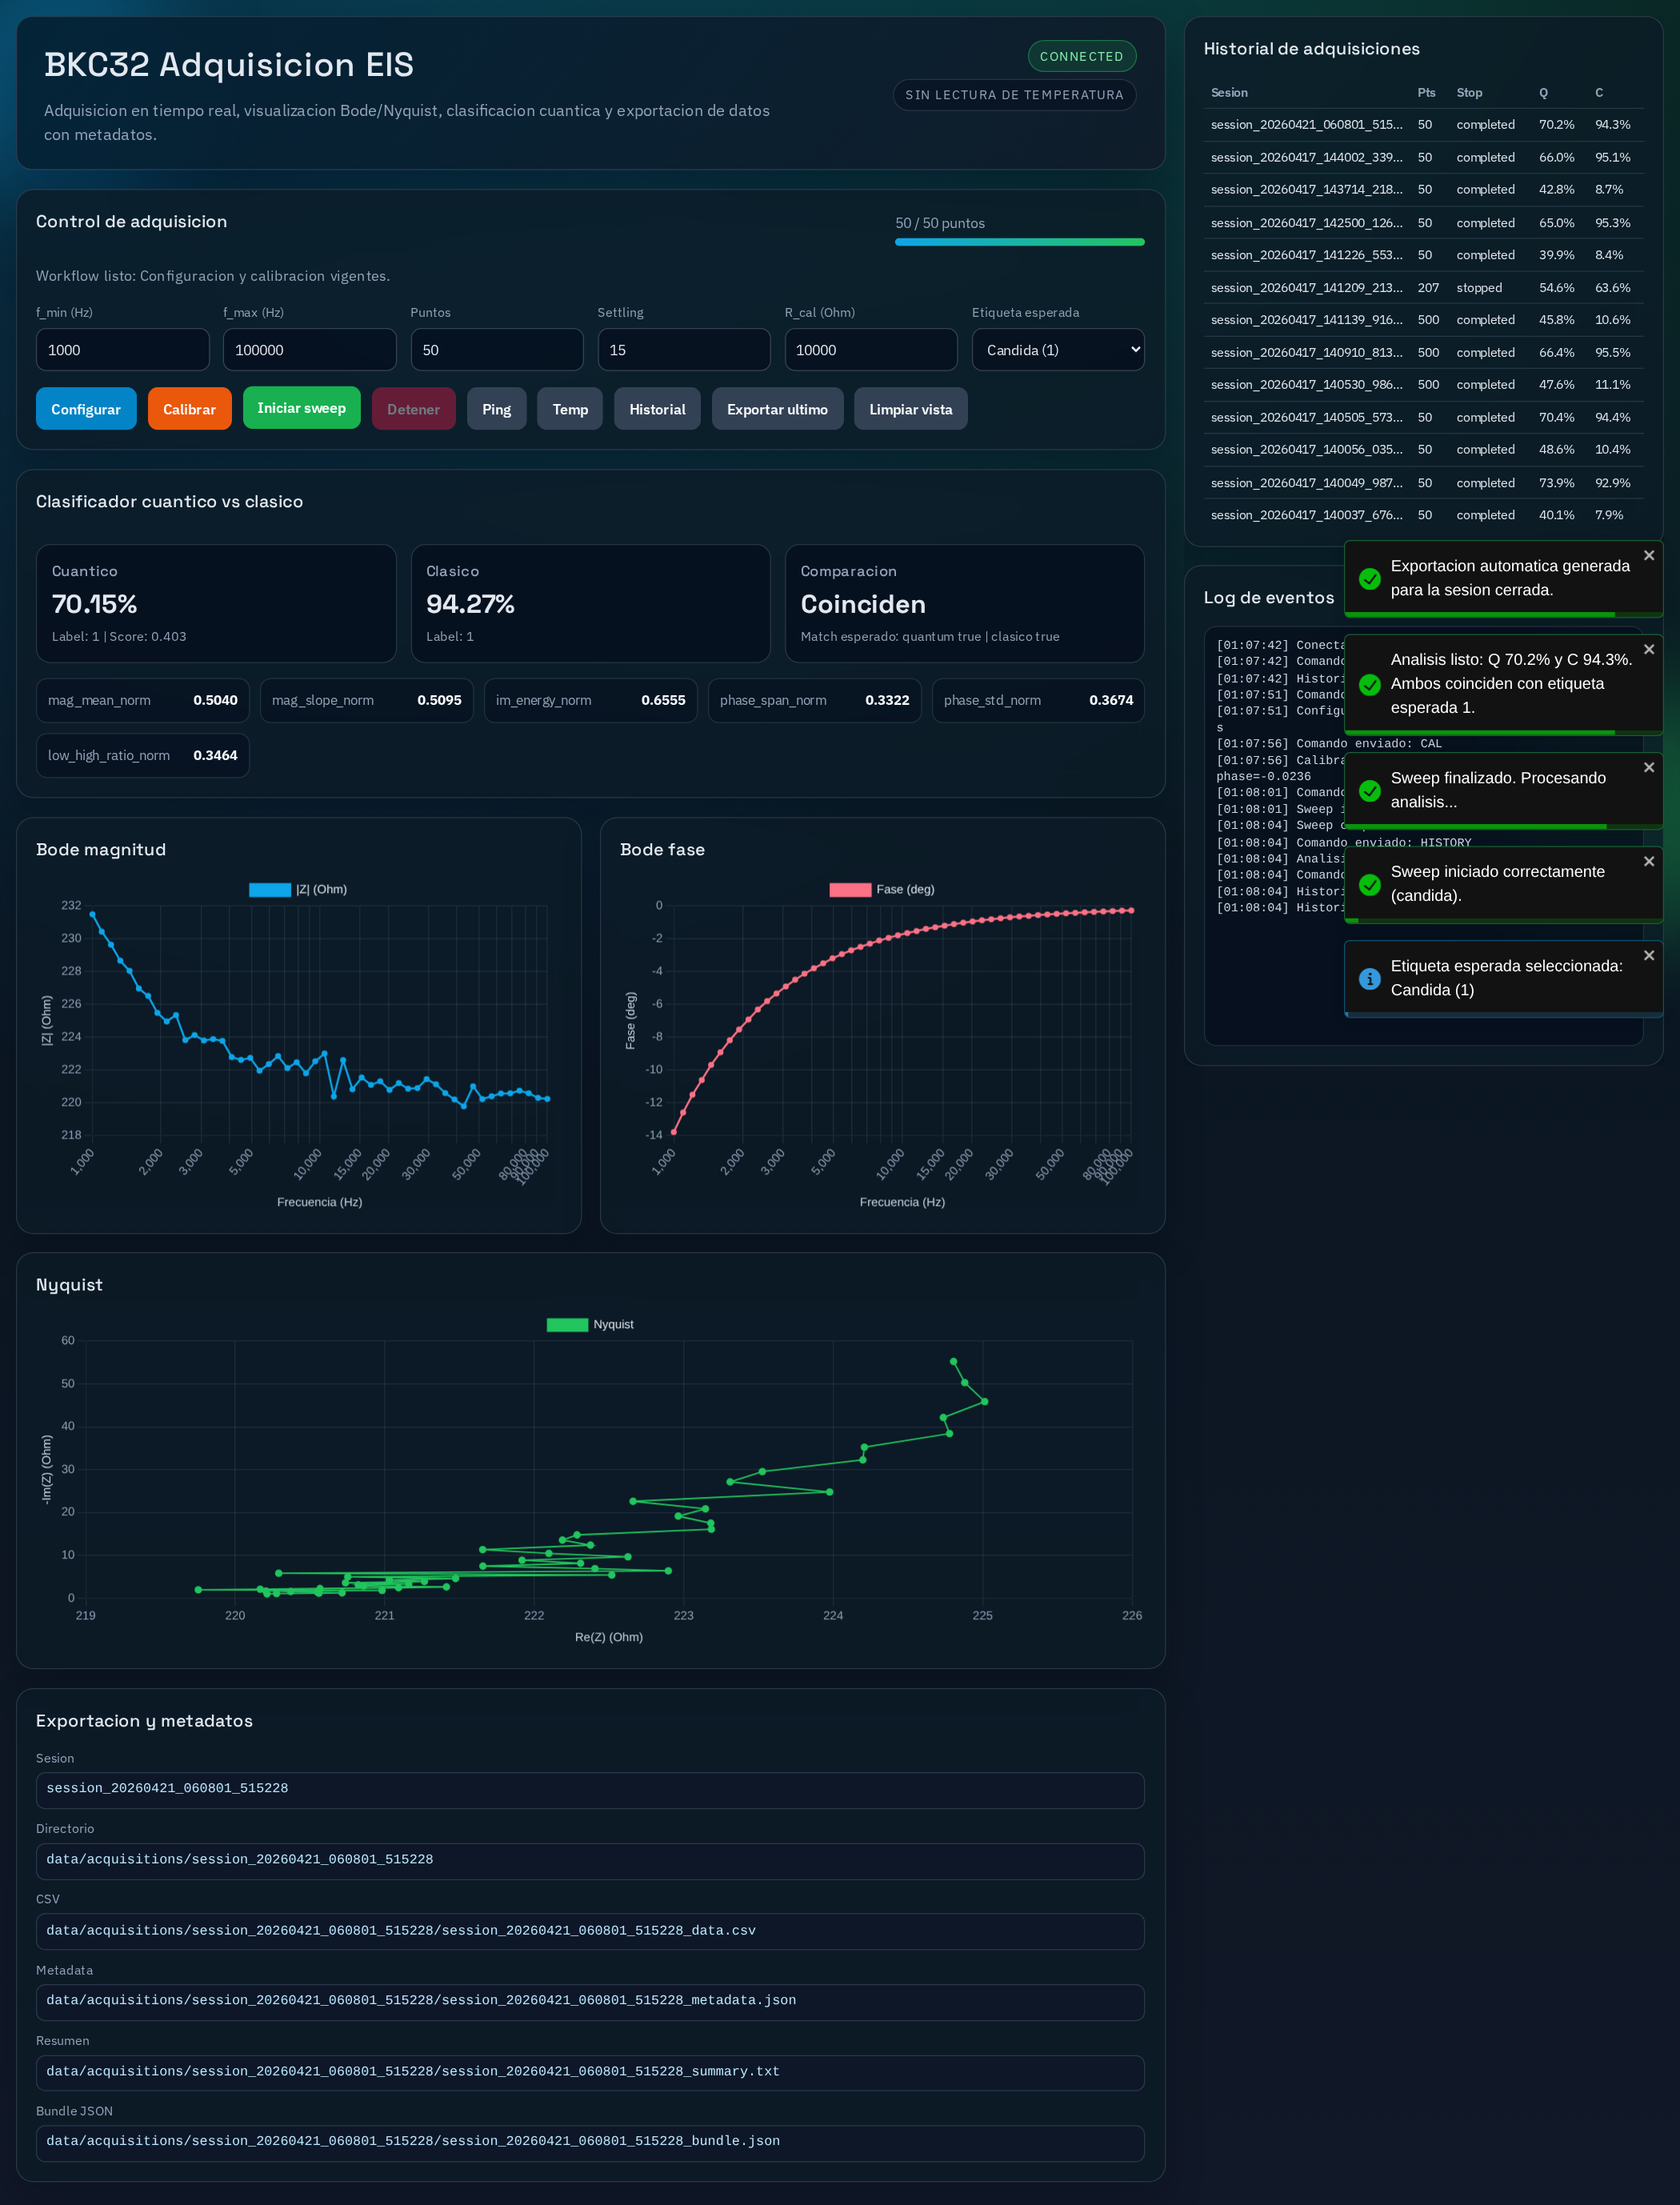
\includegraphics[width=\textwidth]{img/05_sweep_completado_analisis.png}
	\caption[Panel de clasificaci\'{o}n y exportaci\'{o}n al cierre del barrido]{An\'{a}lisis al cierre de un barrido (etiqueta esperada 1), con probabilidades cu\'{a}ntica y cl\'{a}sica, features normalizadas, coincidencia entre modelos y rutas de los archivos exportados autom\'{a}ticamente. Fuente: elaboraci\'{o}n propia.}
	\label{fig:ui-analisis-fase4}
\end{figure}

El umbral de decisi\'{o}n es $0.5$ para ambos clasificadores. Los rangos de interpretaci\'{o}n t\'{i}picos se resumen en la Tabla~\ref{tab:umbrales-clasificacion}.

\begin{table}[ht]
	\centering
	\begin{tabular}{l c p{6.5cm}}
		\hline\hline
		Rango de probabilidad & Etiqueta    & Interpretaci\'{o}n                                \\ [0.5ex]
		\hline
		0\%--20\%             & 0 (Control) & Alta confianza de muestra control                 \\
		20\%--40\%            & 0 (Control) & Confianza moderada de control                     \\
		40\%--50\%            & 0 (Control) & Zona de incertidumbre, tendencia a control        \\
		50\%--60\%            & 1 (Candida) & Zona de incertidumbre, tendencia a candida        \\
		60\%--80\%            & 1 (Candida) & Confianza moderada de candida                     \\
		80\%--100\%           & 1 (Candida) & Alta confianza de candida                         \\
		\hline
	\end{tabular}
	\caption[Interpretaci\'{o}n de probabilidades]{Interpretaci\'{o}n de los porcentajes mostrados por el clasificador cu\'{a}ntico y el cl\'{a}sico. Fuente: elaboraci\'{o}n propia.}
	\label{tab:umbrales-clasificacion}
\end{table}


\chapter{Pruebas de exportaci\'{o}n y trazabilidad}

\section{Sesiones de validaci\'{o}n}

Se ejecutaron dos barridos consecutivos con etiquetas esperadas 1 y 0:
\begin{itemize}
	\item \texttt{session\_20260417\_054612\_940592} (esperada 1)
	\item \texttt{session\_20260417\_054613\_366924} (esperada 0)
\end{itemize}

Ambas sesiones cerraron con \texttt{stop\_reason=completed} y con 40 puntos registrados.

La Figura~\ref{fig:ui-historial} muestra el panel de historial consultable desde la UI. Cada fila presenta el identificador de sesi\'{o}n, el n\'{u}mero de puntos, la raz\'{o}n de parada y las probabilidades Q y C almacenadas.

\begin{figure}[ht]
	\centering
	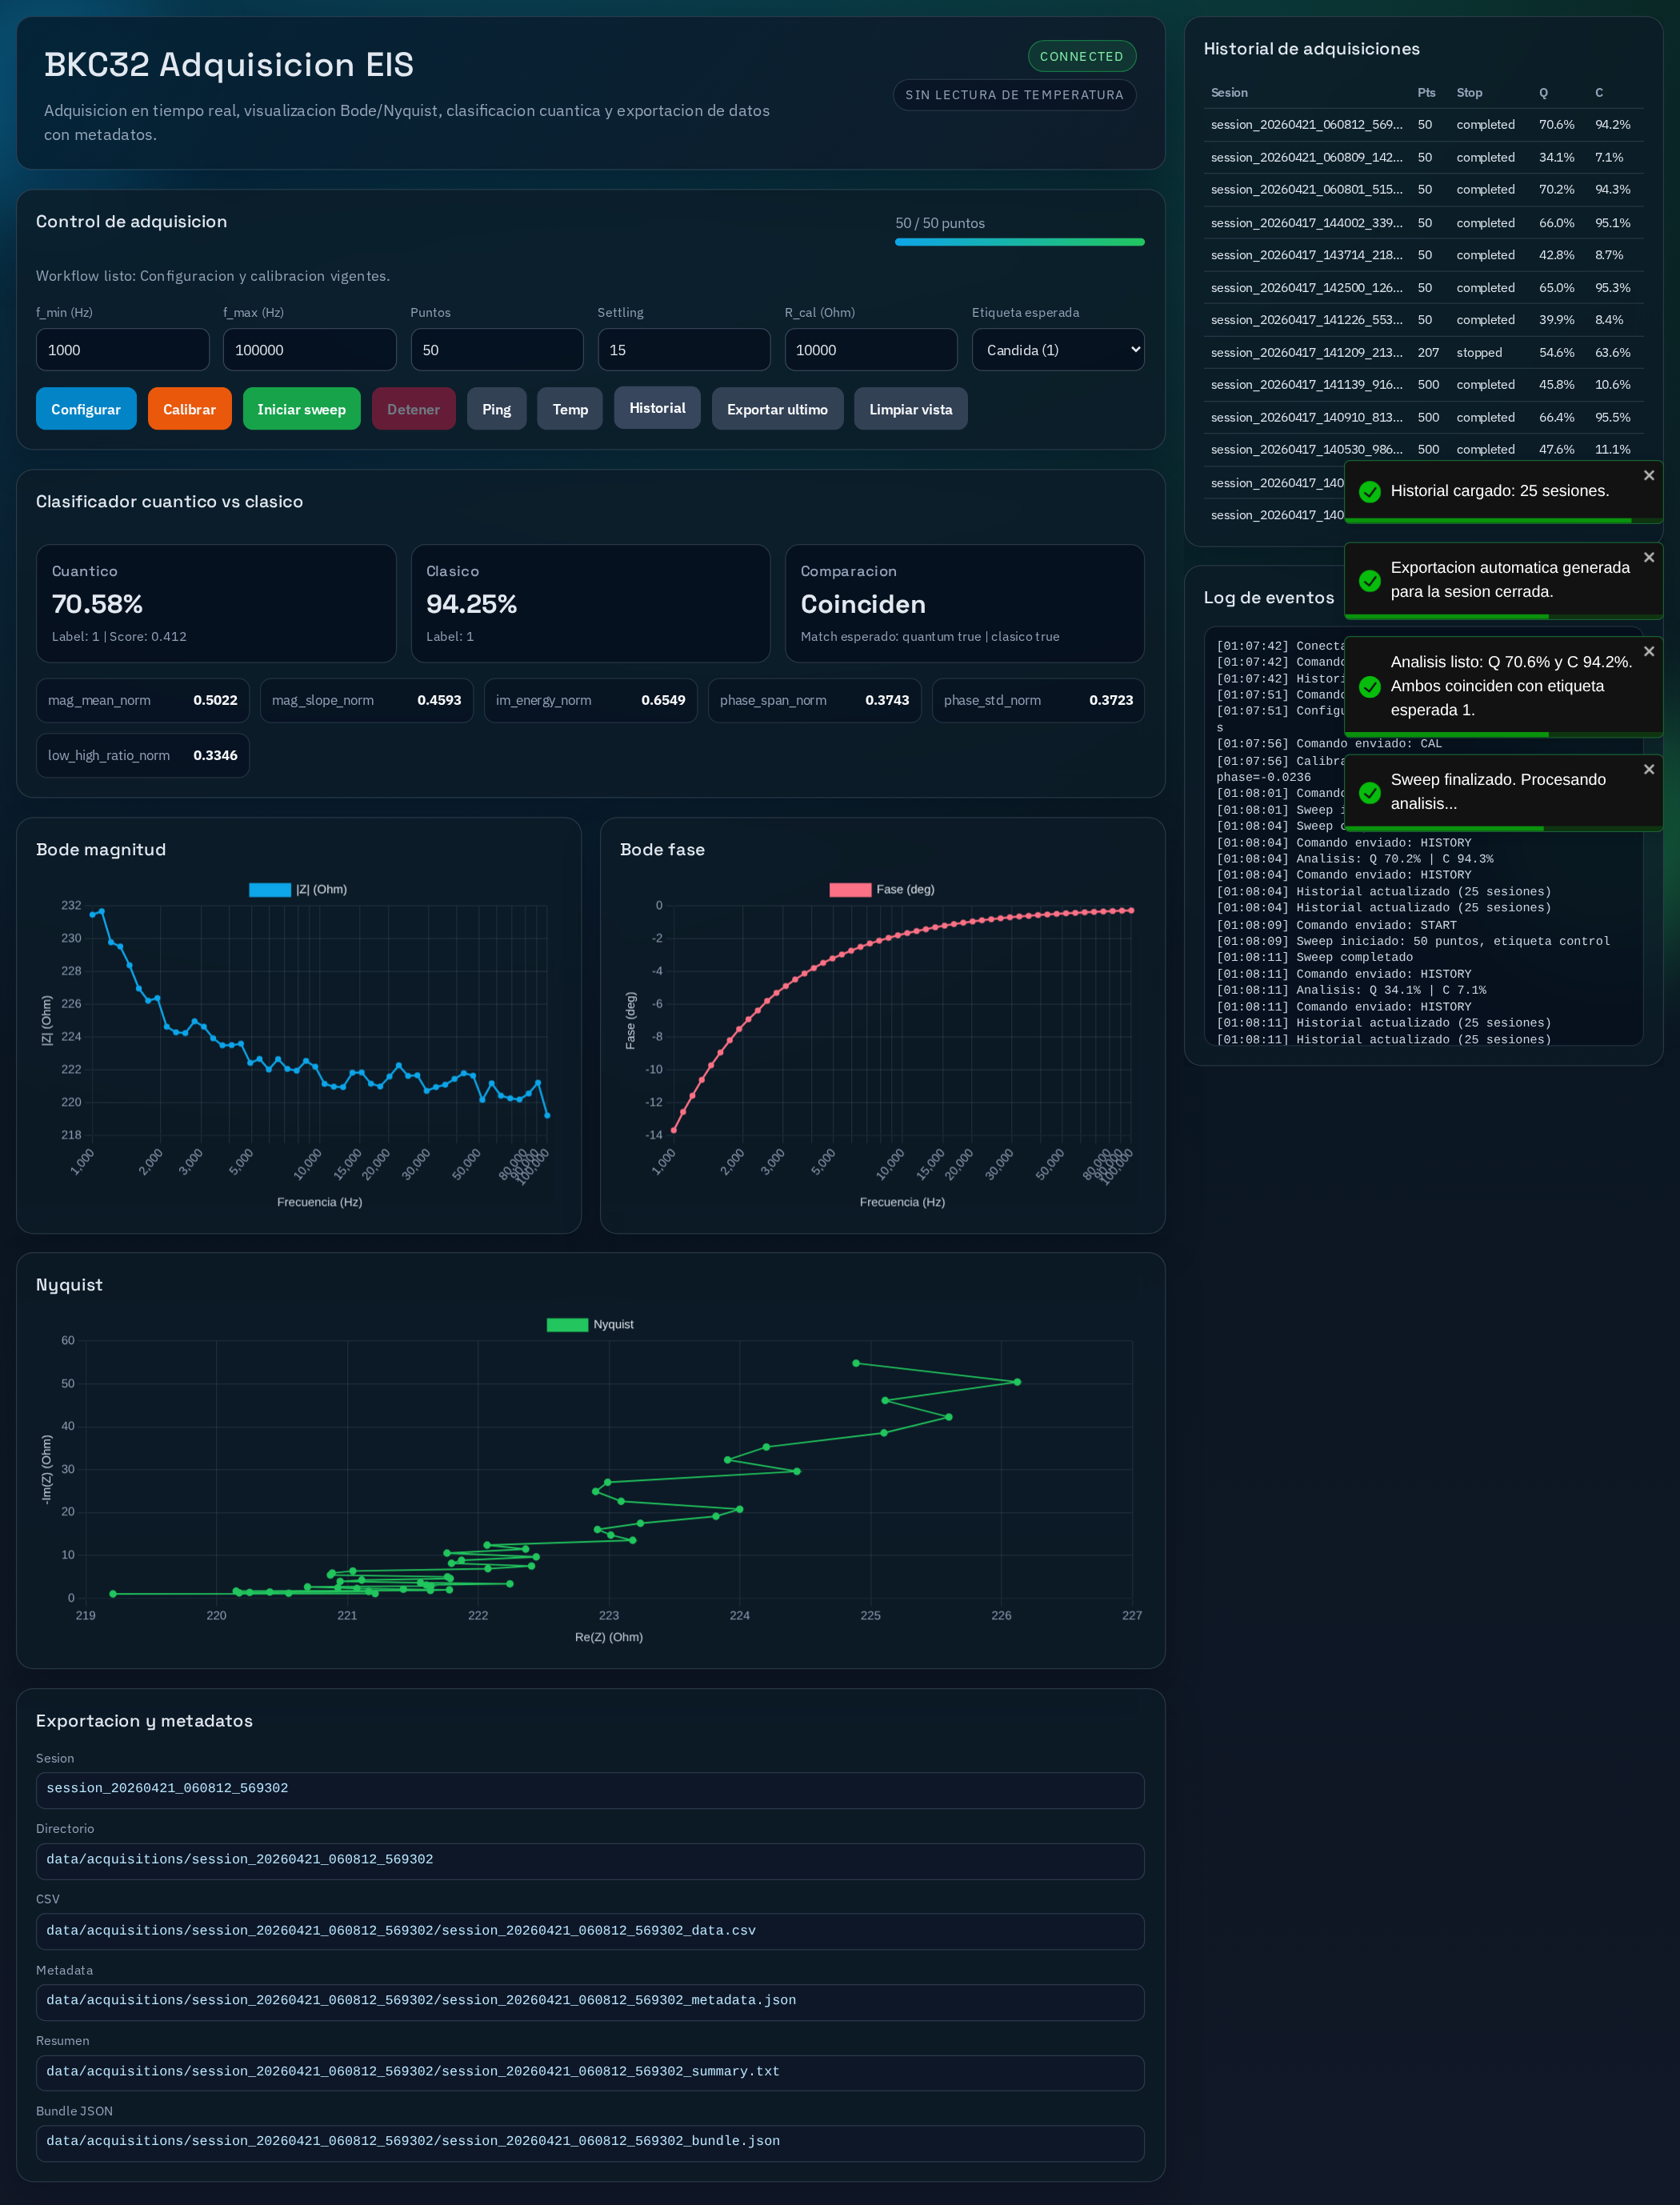
\includegraphics[width=\textwidth]{img/06_historial_sesiones.png}
	\caption[Historial de sesiones en la UI]{Panel de historial con 25 sesiones persistidas: identificador, puntos, raz\'{o}n de cierre y resultados de clasificaci\'{o}n. Fuente: elaboraci\'{o}n propia.}
	\label{fig:ui-historial}
\end{figure}

\section{Resumen de clasificaci\'{o}n y coherencia}

\begin{table}[ht]
	\centering
	\scriptsize
	\begin{tabular}{l c c c c c c}
		\hline\hline
		Sesi\'{o}n & Esperada & Prob. Q  & Label Q & Prob. C  & Label C & Coincidencia \\ [0.5ex]
		\hline
		S1         & 1        & 0.658004 & 1       & 0.949788 & 1       & Q=OK, C=OK   \\
		S2         & 0        & 0.407482 & 0       & 0.080267 & 0       & Q=OK, C=OK   \\
		\hline
	\end{tabular}
	\caption[Validaci\'{o}n de clasificaci\'{o}n por sesi\'{o}n]{Resultados de clasificaci\'{o}n almacenados en metadatos y visualizados en UI (S1: \texttt{...054612\_940592}, S2: \texttt{...054613\_366924}). Fuente: elaboraci\'{o}n propia.}
	\label{tab:validacion-clasificacion-fase4}
\end{table}

\section{Trazabilidad de archivos}

Para la sesi\'{o}n \texttt{session\_20260417\_054612\_940592} se verific\'{o}n los cuatro artefactos:
\begin{itemize}
	\item \texttt{session\_20260417\_054612\_940592\_data.csv}
	\item \texttt{session\_20260417\_054612\_940592\_metadata.json}
	\item \texttt{session\_20260417\_054612\_940592\_summary.txt}
	\item \texttt{session\_20260417\_054612\_940592\_bundle.json}
\end{itemize}

La misma estructura se valid\'{o} para la sesi\'{o}n de control, confirmando consistencia del proceso de exportaci\'{o}n.

La Figura~\ref{fig:ui-exportacion} muestra el panel \textit{Exportaci\'{o}n y metadatos} una vez generados los cuatro artefactos para la sesi\'{o}n m\'{a}s reciente. Las rutas se construyen a partir del identificador temporal y se exponen textualmente para facilitar la inspecci\'{o}n por parte del operador.

\begin{figure}[ht]
	\centering
	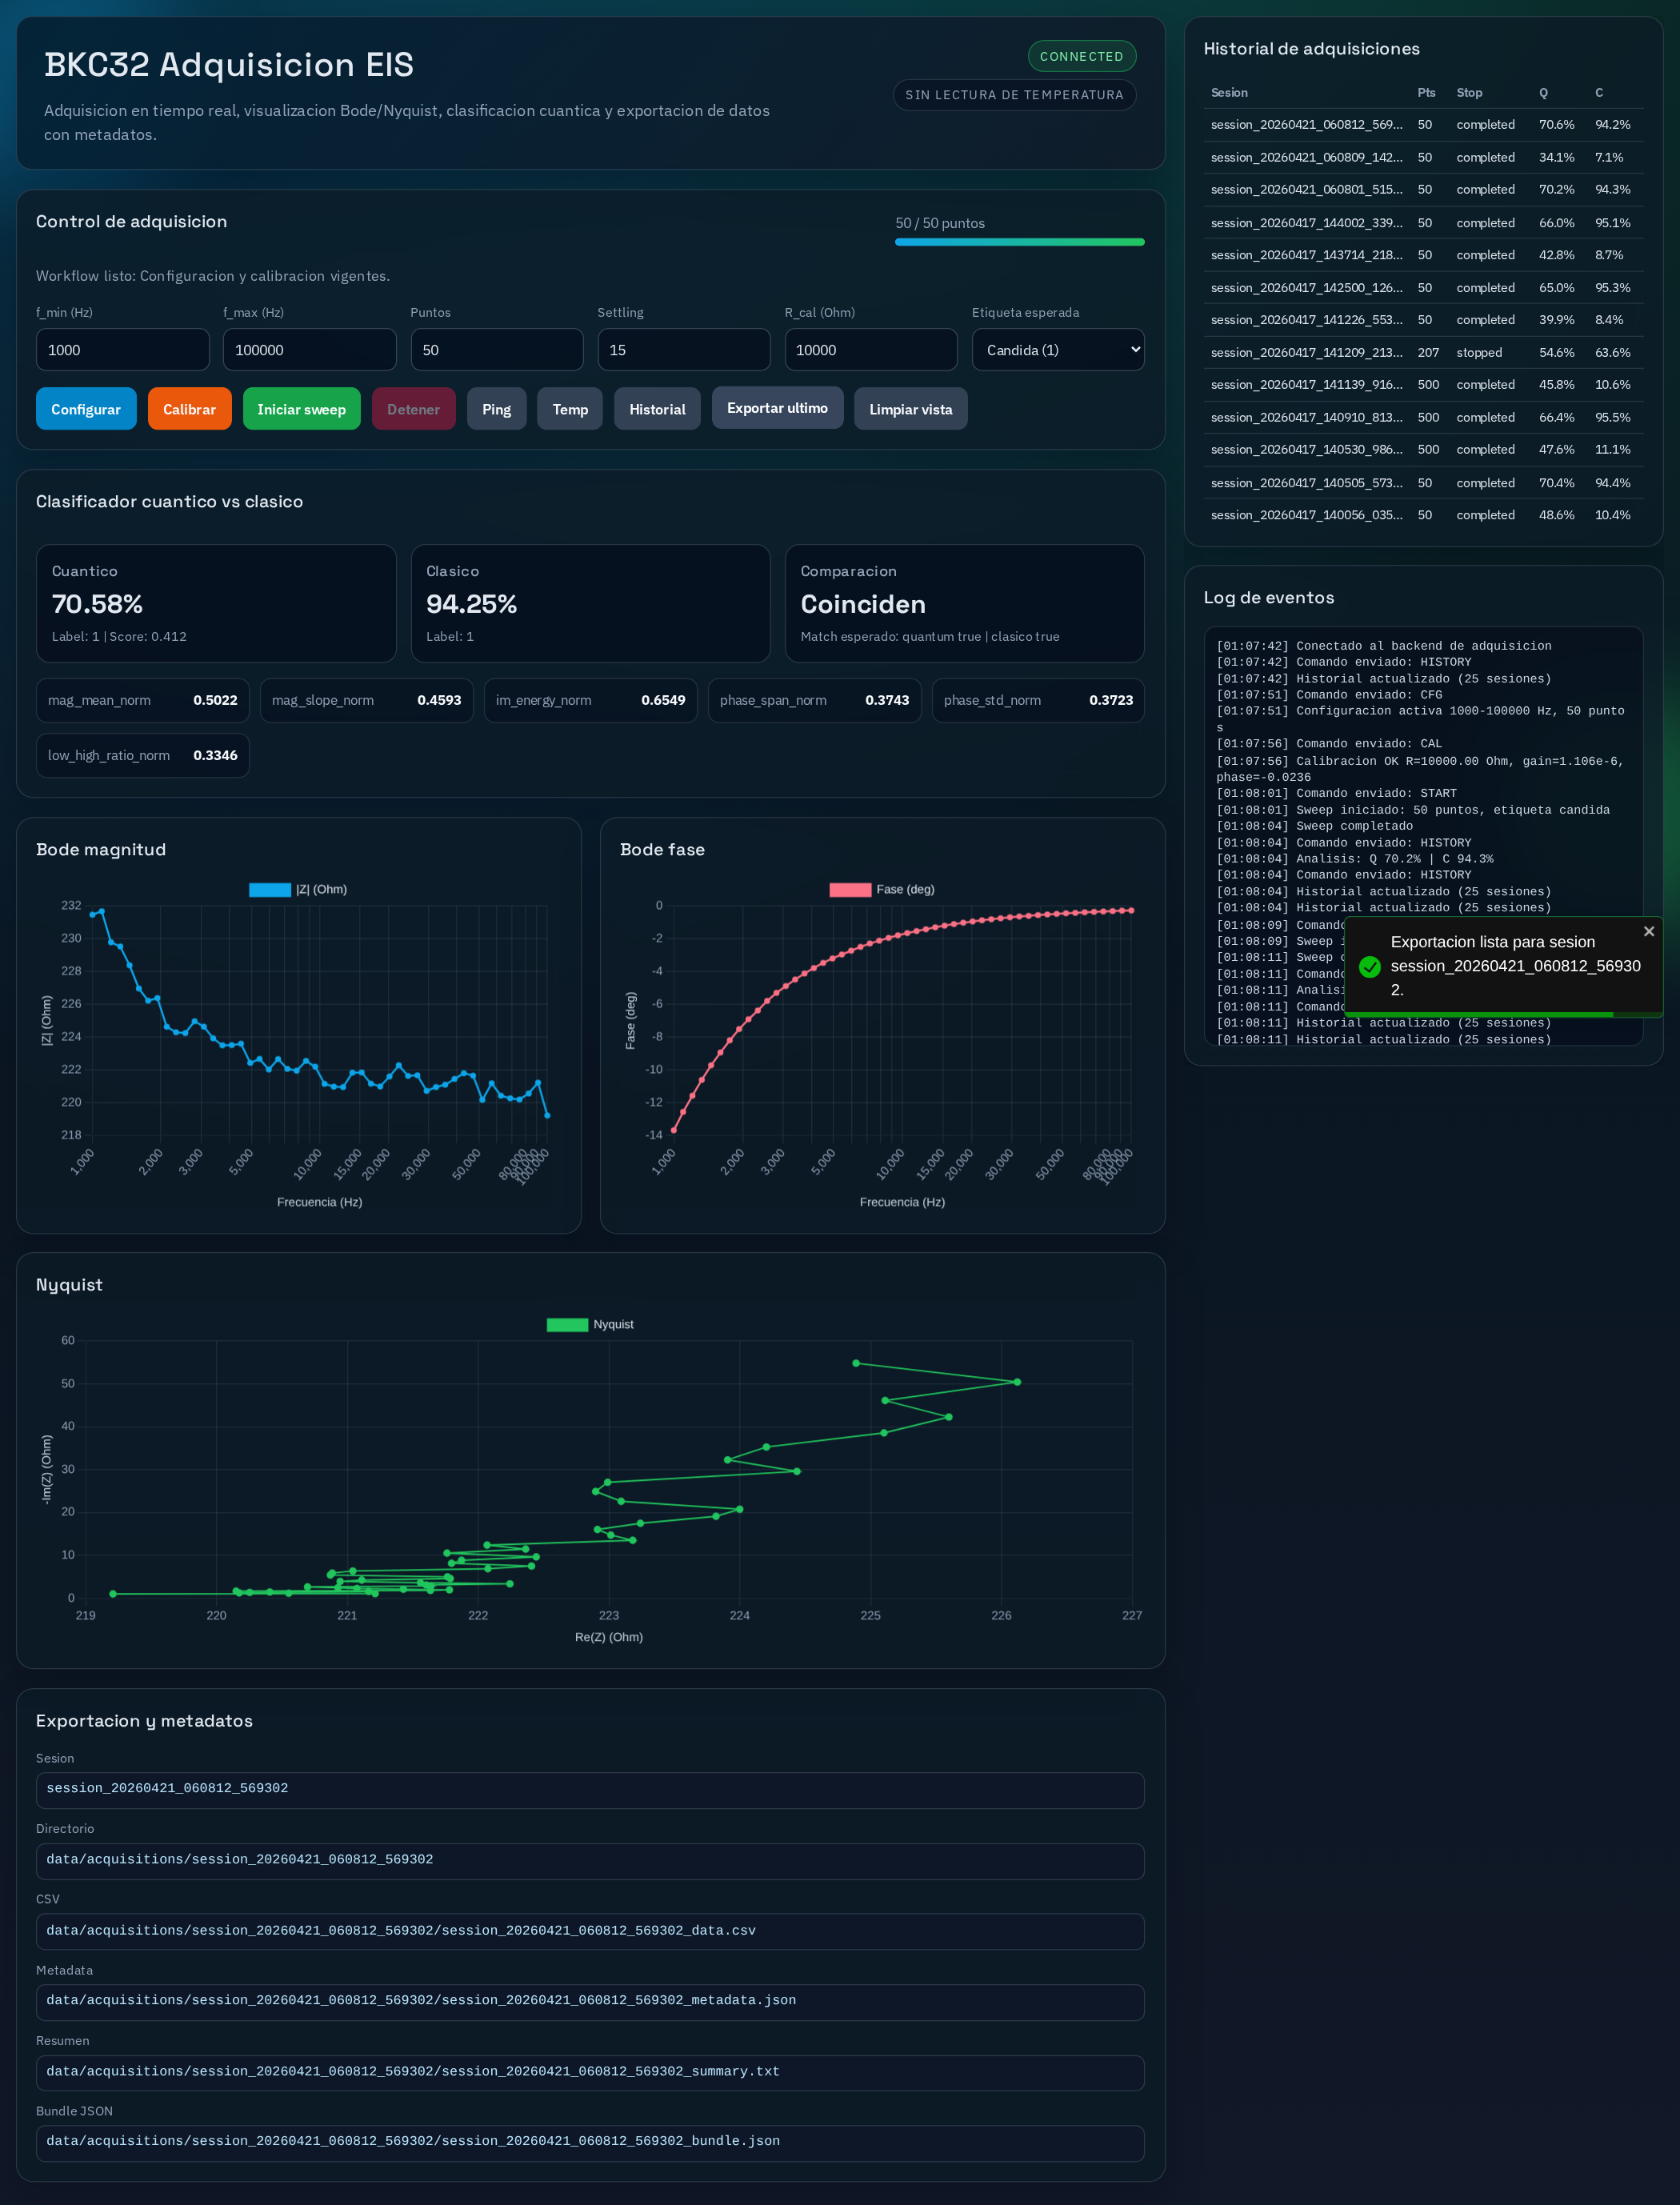
\includegraphics[width=\textwidth]{img/07_exportacion_generada.png}
	\caption[Exportaci\'{o}n generada]{Panel de exportaci\'{o}n con las rutas de CSV, metadata, summary y bundle correspondientes a la \'{u}ltima sesi\'{o}n cerrada. Fuente: elaboraci\'{o}n propia.}
	\label{fig:ui-exportacion}
\end{figure}

\section{Ejemplo de contenido metadata}

El siguiente extracto ilustra la estructura persistida en \texttt{metadata.json}:

\begin{lstlisting}[caption={Estructura simplificada de metadatos por sesi\'{o}n}]
{
  "session_id": "session_20260417_054612_940592",
  "started_at": "2026-04-17T05:46:12.940607+00:00",
  "finished_at": "2026-04-17T05:46:13.363389+00:00",
  "stop_reason": "completed",
  "config": {"fmin": 1000.0, "fmax": 100000.0, "npoints": 40, "settle": 12},
  "calibration": {"gain": 1.1112e-06, "phase": -0.027855, "R_cal": 10000.0},
  "temperature": 26.82,
  "expected_label": 1,
  "analysis": {
    "quantum_probability": 0.658004,
    "quantum_label": 1,
    "classical_probability": 0.949788,
    "classical_label": 1,
    "quantum_match": true,
    "classical_match": true
  }
}
\end{lstlisting}


\chapter{Conclusiones}

La Fase~4 consolida el sistema EIS simulado con capacidades de trazabilidad completas, cumpliendo los objetivos de registro, metadatos y exportaci\'{o}n.

Los aportes principales son:
\begin{itemize}
	\item Modelo de sesi\'{o}n robusto con contexto instrumental y anal\'{i}tico integrado.
	\item Persistencia multi-formato orientada tanto a inspecci\'{o}n humana como a consumo por pipelines autom\'{a}ticos.
	\item Historial consultable desde UI para navegaci\'{o}n de sesiones previas.
	\item Verificaci\'{o}n expl\'{i}cita de clasificaci\'{o}n cu\'{a}ntica y cl\'{a}sica contra etiqueta esperada.
	\item Base lista para siguientes etapas de entrenamiento offline y evaluaci\'{o}n estad\'{i}stica con datasets acumulados.
\end{itemize}

\begin{thebibliography}{99}
	\bibitem[pyserial(2020)]{pyserial} Liechti, C. (2020). pySerial 3.5 Documentation. \url{https://pyserial.readthedocs.io/}
	\bibitem[Python Software Foundation(2026)]{pythonasyncio} Python Software Foundation (2026). \emph{asyncio --- Asynchronous I/O}. \url{https://docs.python.org/3/library/asyncio.html}
	\bibitem[websockets(2026)]{websocketslib} Aymeric Augustin et al. (2026). \emph{websockets 16 Documentation}. \url{https://websockets.readthedocs.io/}
	\bibitem[Havl\'{i}\v{c}ek et al.(2019)]{havlicek2019} Havl\'{i}\v{c}ek, V., C\'{o}rcoles, A. D., Temme, K., Harrow, A. W., Kandala, A., Chow, J. M., \& Gambetta, J. M. (2019). Supervised learning with quantum-enhanced feature spaces. \emph{Nature}, 567(7747), 209--212.
	\bibitem[Bergholm et al.(2022)]{pennylane2022} Bergholm, V., Izaac, J., Schuld, M. et al. (2022). PennyLane: Automatic differentiation of hybrid quantum-classical computations. \emph{arXiv:1811.04968v4}.
\end{thebibliography}

\end{document}
